\section{The Need of Conversational Context}

A prevailing assumption in CGA tasks is that achieving SOTA performance requires models to effectively capture the meaning of utterances within their context and the dynamics of conversations. In this section, we aim to validate this assumption by examining the SOTA performance of RoBERTa-large.

\xhdr{No-Context Setting}

To evaluate whether the models can meaningfully capture the dynamics between conversational utterances, we modify the input context. 
%
Instead of providing the entire conversation context to the model, we feed only the most recent utterance at each timestamp of the conversation. 
%
Formally, in the normal setting, the probability of an event is modeled as $p_{\text{event}} = f(\text{context}(t))$, where $\text{context}(t)$ represents the full history of the conversation up to timestamp $t$. 
%
In contrast, under the No-Context setting, the probability is modeled as $$p_{\text{event}} = f(\text{utterance}(t))$$, where $\text{utterance}(t)$ is the most recent utterance at timestamp $t$. 

\begin{table}[t]
\renewcommand{\arraystretch}{1.0}
    \begin{tabularx}{\linewidth}{|X|}
        \hline
        \textbf{\textit{(1) User1:}} There have been 45 consecutive male presidents and 0 female ones. This gender ratio is extremely imbalanced, and I suggest it's not merely random chance that it's that way.

        \textbf{\textit{(2) User2:}} Women have had the right to vote for many decades and yet they all voted men into office.
        \\
        \multicolumn{1}{|c|}{Label: \textcolor{teal}{Calm}}
        \\ \multicolumn{1}{|c|}{Normal: \textcolor{teal}{Calm}\quad
        No-context: \textcolor{red}{Awry}}
        \\
        \hline

       \textbf{\textit{(1) User1:}} It highly depends on what your religious beliefs are. Muslim? You better not indocrinate your kids.  [...]
       \\
        \textbf{\textit{(2) User2:}}So your argument is based on open Islamophobia?   [...]
        \\
        \multicolumn{1}{|c|}{Label: \textcolor{red}{Awry}} \\
        \multicolumn{1}{|c|}{Normal: \textcolor{red}{Awry}\quad        
        No-context: \textcolor{teal}{Calm}}\\
        
        \hline

    \end{tabularx}

\caption{Examples of conversations where RoBERTa models require the context of current utterances to accurately predict derailment.}
\label{tab:intersection-example}
\end{table}


Table~\ref{tab:intersection-example} presents examples of conversations where RoBERTa models need the conversational context of utterances to accurately predict derailment. 
%
In the first conversation, when the second utterance is considered in isolation, it might be misinterpreted as a critique of women voters' political choices, giving it an escalatory tone. 
%
However, within the full context, its true intent becomes clear: it aims to civilly challenge the argument that the absence of female presidents is rooted in inherent societal or systemic issues.
%
In contrast, in the second example, the phrase "based on open Islamophobia" appears ambiguous when considered in isolation. 
%
It could be interpreted as suggesting that the previous statement merely used Islamophobia as an example to support an argument.
%
However, within the full context, it becomes evident that User2 is criticizing User1, as they perceive User1's argument to be Islamophobic. 
%
Nevertheless, the proportion of test samples where RoBERTa requires context to make correct forecasts is minimal, particularly in CGA-CMV.

\xhdr{Context understanding is not important to SOTA performance} 
%
By evaluating the performance of models under the No-Context setting, we can assess the importance of conversational context to the performance of RoBERTa-large in CGA tasks. 
%
Surprisingly, our experiments demonstrate that the performance of RoBERTa remains largely unchanged, shifting only slightly from 68.4\% to 67.8\% on CGA-CMV and from 68.1\% to 65.4\% on CGA-Wiki. 
%
This suggests that conversational context may not significantly impact the SOTA performance of RoBERTa on CGA tasks.
%
Moreover, as shown in Figure~\ref{fig:convo_level_changes}, most conversation-level forecast probabilities (defined as the highest utterance-level forecast in each conversation) remain largely unchanged even with the absence of the conversational context in the No-Context setting.
\begin{figure}[ht]
    \centering
    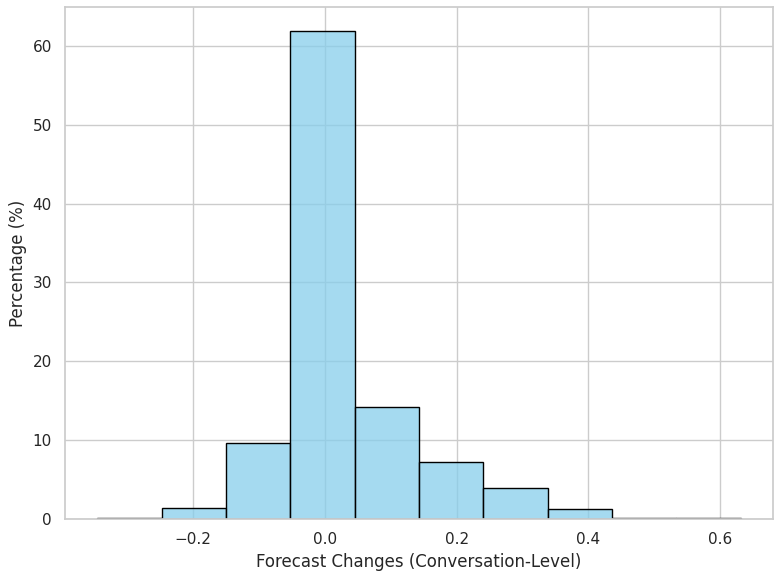
\includegraphics[width=\linewidth]{figures/convo_level_changes.png}
    \caption{
        Changes in RoBERTa model conversation-level forecast probabilities due to the absence of conversational context (No-Context Setting).}
    \label{fig:convo_level_changes}
\end{figure}
\xhdr{RQ2. SOTA models do leverage context when making forecasts}
However, finding in previous analysis does not suggest that RoBERTa models primarily disregard conversational context when predicting conversation outcomes. 
%
To further explore this, we analyze the model's predictions at the utterance level. 
%
Specifically, to determine whether the models utilize context in their predictions, we examine the forecast probabilities that exhibit the most significant changes within each conversation when the conversational context is removed. 
%
Our analysis, presented in Figure~\ref{fig:utt_level_changes}, reveals that the absence of context significantly impacts the forecasts of RoBERTa models at the utterance level.

\begin{figure}[ht]
    \centering
    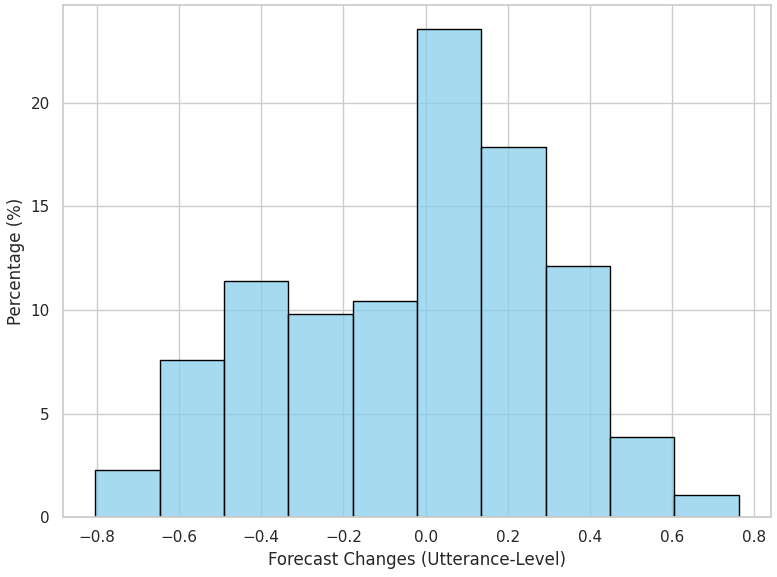
\includegraphics[width=\linewidth]{figures/utt_level_changes.png}
    \caption{Most significant changes in RoBERTa model utterance-level forecast probabilities within each conversation due to the absence of conversational context (No-Context Setting).}
    \label{fig:utt_level_changes}
\end{figure}

Building on this observation, we investigate whether the absence of context affects the performance of models at the utterance level. 
%
Due to the nature of CGA, ground-truth labels at the utterance level are only available for the timestamp preceding the final utterance of a conversation, where personal attacks may arise. 
%
Surprisingly, our evaluation reveals a notable decline in performance: accuracy drops from 69.9\% to 63.3\% on CGA-CMV and from 68.3\% to 61.1\% on CGA-Wiki. 
%
This performance gap is notably larger than the one observed at the conversation level.

